% VistaQA Zero-Shot Challenge system report.
% Format and requirements: docs/submission.md#report-format.
% Numbers and their sources: report/draft_ru.md (source comments) and docs/results.md.
\documentclass{article}

% Numeric citations keep tables and the four-page body compact.
\PassOptionsToPackage{numbers,sort&compress}{natbib}
% Submission mode (line numbers, "Submitted to" notice); use [sglblindworkshop, final] for the camera-ready version.
\usepackage[sglblindworkshop]{neurips_2026}
\workshoptitle{Grounded and Faithful Vision-Language Models for Real-World Deployment}

\usepackage[utf8]{inputenc}
\usepackage[T1]{fontenc}
\usepackage{hyperref}
\usepackage{url}
\usepackage{booktabs}
\usepackage{tabularx}
\usepackage{amsmath}
\usepackage{amsfonts}
\usepackage{microtype}
\usepackage{xcolor}
\usepackage{graphicx}
\usepackage{listings}
\usepackage{tikz}
\usetikzlibrary{arrows.meta, positioning, fit, backgrounds}

\lstset{basicstyle=\ttfamily\scriptsize, breaklines=true, columns=fullflexible, keepspaces=true, frame=single}

\newcommand{\ci}[2]{[#1,\,#2]}
% Public repository for code, predictions and evaluation (docs/submission.md#repository).
\newcommand{\repourl}{https://github.com/yhn112/vistaqa-premise-check}

\title{Answer, Segment, Then Check the Premise:\\A Zero-Shot VLM and SAM~3 System for VistaQA}

\author{%
  Michael Diskin \\
  HSE University \\
  \texttt{michael.s.diskin@gmail.com} \\
  Team: YHN112
}

\begin{document}

\maketitle

\begin{abstract}
  Grounded visual question answering asks a model not only to answer, but to show the pixels that justify the answer,
  and to say so when the question asks about something that is not there.
  We approach the VistaQA Zero-Shot Challenge with a deliberately simple, training-free system:
  a strong reasoning vision-language model decides what to answer and where the evidence is,
  and SAM~3 turns its boxes into masks.
  The one addition that earned its place is a premise check that doubts the question rather than the answer:
  in a fresh context, the model lists what the question takes for granted and checks each assumption against the image,
  overriding the answer only when an assumption clearly fails.
  Heavier machinery did not pay off on our development sets built from public data:
  mask verification, evidence re-localization, click prompts for SAM~3, an active visual audit and voting over repeated runs.
  Additional checking tended to reinforce mistakes rather than fix them,
  and the errors that remain are often about which object counts as evidence rather than where its boundary lies.
  The final system reaches a GROVE of 75.31 ($\varepsilon=0.01$) on the 1157 public VistaQA samples.
\end{abstract}

\section{Introduction}

VistaQA~\citep{vistaqa} asks a system to answer a question about an image
and to mark the pixels of the objects that support the answer;
for a question with a false premise (314 of the 1157 samples), it should state what is absent and return no masks.
We split the work between two off-the-shelf models:
a reasoning VLM decides what to answer and where to look, and SAM~3~\citep{sam3} draws the masks from its boxes.
One pipeline serves all six domains (AV, indoor, outdoor, math, robotics, science) without domain routing or training.
Of all additions to this base pass we adopted only one, a premise check, selected on our development sets (Section~\ref{sec:validation});
several other natural extensions did not help (Section~\ref{sec:negative}).

\section{Task and metric}
\label{sec:task}

A sample is an image and a question of one of six task types
(attribute, comparison, counting, identification, OCR, spatial); a prediction is a text answer and a list of instance masks.
The answer score $S_a\in\{0,1\}$ is the verdict of an LLM judge given the question, reference, prediction, task type and domain.
For the mask score $S_m$, masks are matched by the Hungarian algorithm on IoU,
and the matched IoUs are summed and divided by $\max(k,m)$ for $k$ reference and $m$ predicted masks
($S_m=1$ if both lists are empty and 0 if exactly one is).
GROVE averages $\sqrt{\max(S_a,\varepsilon)\max(S_m,\varepsilon)}$ over samples.
The paper uses a Qwen2.5-14B judge and $\varepsilon=0.1$; the official code, which we use,
defaults to Qwen2.5-72B-Instruct~\citep{qwen25} (here through OpenRouter) and to our primary $\varepsilon=0.01$.

\section{System}
\label{sec:system}

\begin{figure}[t]
  \centering
  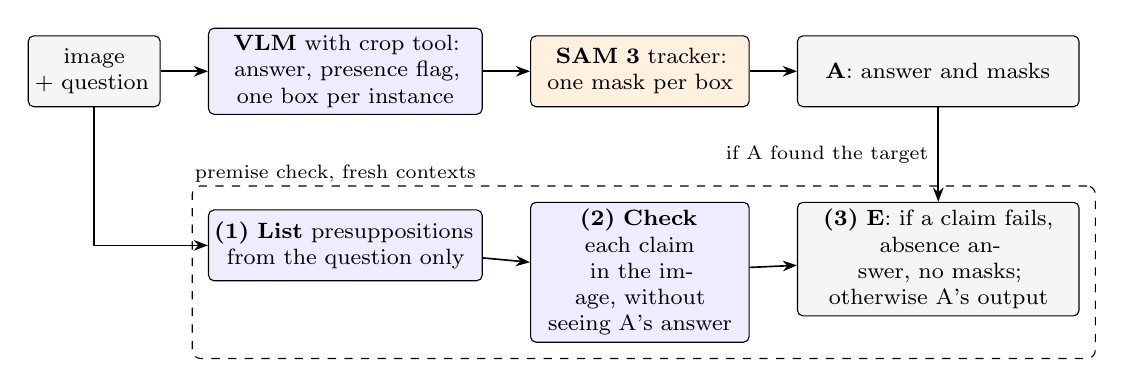
\begin{tikzpicture}[
      font=\footnotesize,
      node distance=3mm and 6mm,
      box/.style={draw, rounded corners=2pt, align=center, inner sep=2.5pt, minimum height=9mm, text width=#1},
      arr/.style={-{Stealth[length=1.8mm]}, semithick}]
    \node[box=1.5cm, fill=gray!8] (in) {image\\+ question};
    \node[box=3.3cm, fill=blue!7, right=of in] (ans) {\textbf{VLM} with crop tool:\\answer, presence flag,\\one box per instance};
    \node[box=2.6cm, fill=orange!12, right=of ans] (sam) {\textbf{SAM~3} tracker:\\one mask per box};
    \node[box=3.4cm, fill=gray!8, right=of sam] (a) {\textbf{A}: answer and masks};
    \draw[arr] (in) -- (ans);
    \draw[arr] (ans) -- (sam);
    \draw[arr] (sam) -- (a);
    \node[box=3.3cm, fill=blue!7, below=12mm of ans] (list) {\textbf{(1) List} presuppositions\\from the question only};
    \node[box=2.6cm, fill=blue!7, below=12mm of sam] (check) {\textbf{(2) Check} each claim\\in the image, without\\seeing A's answer};
    \node[box=3.4cm, fill=gray!8, below=12mm of a] (dec) {\textbf{(3) E}: if a claim fails,\\absence answer, no masks;\\otherwise A's output};
    \draw[arr] (list) -- (check);
    \draw[arr] (check) -- (dec);
    \draw[arr] (a) -- node[left, font=\scriptsize] {if A found the target} (dec);
    \draw[arr] (in.south) |- (list.west);
    \begin{scope}[on background layer]
      \node[draw, dashed, rounded corners=3pt, inner sep=2mm, fit=(list) (check) (dec),
        label={[font=\scriptsize, anchor=south west, inner sep=1pt]north west:premise check, fresh contexts}] {};
    \end{scope}
  \end{tikzpicture}
  \caption{System overview: the base pass A (top) and the premise check that completes the full system E (bottom).}
  \label{fig:system}
\end{figure}

\subsection{Answer and evidence boxes}

The VLM is gpt-6.1-sol at reasoning effort xhigh,
called by a PydanticAI~\citep{pydanticai} agent through its \texttt{openai-codex:} provider, i.e.\ the Codex backend.
The image is sent at its metadata resolution without downscaling.
The model has a \texttt{crop} tool to cut out and inspect a region;
crops whose long side is below 1024\,px are enlarged to 1024\,px.
The output is JSON validated against a Pydantic schema:
the answer, a \texttt{target\_present} flag and a list of evidence entries, each with a label and a box in original-image pixels.

The prompt (Appendix~\ref{app:prompts}) asks for a short answer,
and for an absence answer with no evidence when anything the question refers to is missing or the requested count is zero.
The evidence is what the question asks about: only the selected object in comparisons, one entry per counted instance,
the named object rather than its label, no reference or context objects, and nothing when unsure.

\subsection{Evidence masks with SAM~3}

Each box is passed separately as a box prompt to the tracker (promptable visual segmentation) head of SAM~3~\citep{sam3}
(\texttt{facebook/sam3} in transformers 5.22.2, torch 2.15.0, float32, Apple MPS),
which returns one mask per box (multimask output off) at mask threshold 0.5.
Masks are produced at the metadata resolution, which is also the resolution of the reference masks.

\subsection{Premise check}
\label{sec:premise}

The base pass (A) sometimes answers a false-premise question as if the object were present:
on our final dev mix (Section~\ref{sec:selection}) it returned masks for 21 of the 241 questions without reference masks.
The full system (E) therefore adds two calls to the same model in fresh contexts (Figure~\ref{fig:system}).
\textbf{(1)} From the question alone, the model lists what it takes for granted as short claims
about objects, attributes, relations, and text or information, never the unknown the question asks for.
\textbf{(2)} With the image, the question and the claims but not A's answer, so that it is not anchored to it,
the model returns \emph{holds}, \emph{fails} or \emph{unclear} for each claim with the observation behind it.
A claim fails only when the image clearly shows the opposite;
a similar object with a different attribute does not make an attribute claim hold.
\textbf{(3)} If any claim fails, the checker's absence sentence (``There is no pink bucket in the image.'') replaces A's output;
otherwise A's answer and masks are kept, and an empty detector output alone never establishes absence.
The check raises the mean number of logical model requests per VistaQA image from 2.56 to 5.20;
Appendix~\ref{app:implementation} describes orchestration, retries and caching.

\section{Development protocol}
\label{sec:dev}

\subsection{Development sets}

We measure changes on our own dev sets in VistaQA format, built from public data and synthetic figures (Table~\ref{tab:devsets});
this report uses only their dev splits.
Images from real sources were checked against the VistaQA images by comparing pixels only
(SIFT matching, a RANSAC similarity fit and correlation after alignment),
and all matches were excluded: 186 AI2D diagrams, 13 nuImages frames, 31 DROID frames and 4 SA-1B images.

\begin{table}[t]
  \caption{Development sets; the last column counts questions in the dev split.}
  \label{tab:devsets}
  \centering
  \footnotesize
  \begin{tabularx}{\linewidth}{@{}llXr@{}}
    \toprule
    Set (domains) & Images & Questions and masks & dev \\
    \midrule
    SA-Co (in-/outdoor) & SA-1B~\citep{sam} via SA-Co/Gold~\citep{sam3} & templates; reviewed questions; OCR from SA-Text~\citep{satext} & 258 \\
    math & synthetic (ours) & programmatic answers and masks & 233 \\
    science & AI2D~\citep{ai2d} & templates; reviewed part questions on SAM~3 masks & 181 \\
    AV & nuImages~\citep{nuscenes} & templates on nuImages masks; reviewed questions & 115 \\
    robotics & DROID~\citep{droid}, RoboRefIt~\citep{roborefit} & reviewed questions; SAM~3 / human masks & 136 \\
    \bottomrule
  \end{tabularx}
\end{table}

Reviewed questions were written by Claude Opus 5.5 agents from sheets of candidate masks under explicit criteria
(unambiguous evidence, one task type, a short answer)
and checked blindly by another agent (all false-premise questions, all counts of four or more and a quarter of the rest).
In the final mix, 241 of 923 questions (26.1\%) have a false premise.

\subsection{Selection criterion}
\label{sec:selection}

The primary metric is the mean GROVE over six equally weighted domains on a fixed mix of 923 dev questions
(SA-Co contributes indoor and outdoor); the mean over questions is secondary.
Variants share questions, judge and cached verdicts;
intervals come from a paired bootstrap (10{,}000 resamples of questions within domains, seed 0).
A variant that changes only later stages pins the base run's answers and masks (E reuses a completed A run),
so differences are not confounded with model resampling.
Decision rules were fixed at $\varepsilon=0.1$, for larger comparisons before inference;
at the reported $\varepsilon=0.01$, all signs and whether intervals include zero are the same.

\section{Results}
\label{sec:results}

\subsection{VistaQA}

\begin{table}[t]
  \caption{VistaQA, 1157 samples, Qwen2.5-72B-Instruct judge; E reuses A's answers and masks.
    Left: overall scores. Right: GROVE ($\varepsilon=0.01$) by domain and task type, A $\rightarrow$ E,
    from the official evaluator's standard breakdown.}
  \label{tab:vistaqa}
  \centering
  \footnotesize
  \setlength{\tabcolsep}{4pt}
  \begin{minipage}[t]{0.44\linewidth}
    \centering
    \begin{tabular}{lrr}
      \toprule
      Measure & A & E (ours) \\
      \midrule
      \textbf{GROVE, $\varepsilon=0.01$} & 73.68 & \textbf{75.31} \\
      GROVE, $\varepsilon=0.1$ & 76.83 & 78.29 \\
      $S_a$ & 80.81 & 82.28 \\
      $S_m$ & 75.60 & 77.08 \\
      $S_m$, false premise (314) & 72.29 & 84.71 \\
      $S_m$, grounded (843) & 76.82 & 74.24 \\
      Requests / image & 2.56 & 5.20 \\
      \bottomrule
    \end{tabular}
  \end{minipage}\hfill
  \begin{minipage}[t]{0.54\linewidth}
    \centering
    \begin{tabular}{lrlr}
      \toprule
      Domain & A $\rightarrow$ E & Task & A $\rightarrow$ E \\
      \midrule
      AV & 77.15 $\rightarrow$ 78.47 & attribute & 76.12 $\rightarrow$ 79.23 \\
      indoor & 71.80 $\rightarrow$ 75.21 & comparison & 78.42 $\rightarrow$ 79.04 \\
      math & 74.35 $\rightarrow$ 75.01 & counting & 76.63 $\rightarrow$ 78.34 \\
      outdoor & 76.09 $\rightarrow$ 78.60 & identification & 72.52 $\rightarrow$ 74.62 \\
      robotics & 54.93 $\rightarrow$ 56.56 & OCR & 74.86 $\rightarrow$ 73.63 \\
      science & 87.72 $\rightarrow$ 87.73 & spatial & 64.22 $\rightarrow$ 67.29 \\
      \bottomrule
    \end{tabular}
  \end{minipage}
\end{table}

Table~\ref{tab:vistaqa} gives the VistaQA scores.
E minus A is $+1.63$ GROVE at $\varepsilon=0.01$, paired bootstrap 95\% CI \ci{+0.41}{+2.84}
($+1.46$, \ci{+0.35}{+2.56} at $\varepsilon=0.1$).
The submitted predictions are those of E; they and their evaluation are linked in Section~\ref{sec:resources}.
Appendix~\ref{app:posthoc} gives a post-hoc analysis of how the premise check changed the VistaQA answers.

\subsection{Our validation}
\label{sec:validation}

We selected E on our dev data: it scored best among the variants A--E on early versions of the dev sets,
and later additions gave no significant gain over it on the final mix (Section~\ref{sec:negative}).
Table~\ref{tab:validation} shows the effect of the premise check on the final mix.

\begin{table}[t]
  \caption{A and E on the final dev mix (923 questions, $\varepsilon=0.01$): GROVE / $S_a$ / $S_m$, and E $-$ A in GROVE with a paired 95\% CI.}
  \label{tab:validation}
  \centering
  \footnotesize
  \begin{tabular}{lllr}
    \toprule
    Level & A & E (ours) & E $-$ A \\
    \midrule
    \textbf{Mean over 6 domains} & 84.29 / 91.35 / 83.57 & \textbf{85.82} / 92.88 / 85.13 & \textbf{+1.52} \ci{+0.49}{+2.73} \\
    Mean over questions & 85.45 / 93.28 / 83.86 & 86.54 / 94.37 / 84.97 & +1.09 \ci{+0.26}{+1.94} \\
    \midrule
    AV (115) & 79.83 / 87.83 / 79.55 & 81.56 / 89.57 / 81.29 & +1.72 \ci{0.00}{+4.30} \\
    indoor (62) & 78.15 / 82.26 / 82.62 & 81.35 / 85.48 / 85.85 & +3.19 \ci{0.00}{+7.98} \\
    math (233) & 84.20 / 98.71 / 80.01 & unchanged & 0.00 \\
    outdoor (196) & 87.21 / 91.84 / 87.53 & 87.74 / 92.35 / 88.11 & +0.54 \ci{-0.94}{+2.53} \\
    robotics (136) & 84.16 / 89.71 / 83.30 & 87.85 / 93.38 / 87.08 & +3.69 \ci{-0.55}{+8.04} \\
    science (181) & 92.20 / 97.79 / 88.42 & unchanged & 0.00 \\
    \bottomrule
  \end{tabular}
\end{table}

E changed 16 answers, 13 correctly (81\%).
The share of false-premise questions that receive masks fell from 8.7\% (21 of 241) to 3.3\% (8),
while 3 of the 682 grounded questions received an incorrect absence answer (none for A).
E changed nothing in math, where A already rejects every false premise, or in science, where the check missed A's three errors.
Dev scores are not directly comparable with VistaQA: images and questions differ, and some dev reference masks are SAM~3 masks.

\subsection{What did not help}
\label{sec:negative}

\begin{table}[t]
  \caption{Changes relative to E on the final dev mix (mean GROVE over domains, $\varepsilon=0.01$; E: 85.82), with paired 95\% CIs.
    All were measured on dev data with E fixed; VistaQA was not run for them.}
  \label{tab:negative}
  \centering
  \footnotesize
  \begin{tabularx}{\linewidth}{@{}lXr@{}}
    \toprule
    Variant & What changes & $\Delta$ vs.\ E \\
    \midrule
    Re-localization & the VLM localizes the evidence again for the fixed answer & $-0.31$ \ci{-1.04}{+0.39} \\
    SAM~3 clicks & the VLM places positive and negative points in the fixed boxes & $+0.09$ \ci{-0.11}{+0.33} \\
    Clicks + multimask & as above, keeping the mask with the highest predicted IoU & $+0.17$ \ci{-0.10}{+0.48} \\
    Full chain & re-localization, clicks and multimask & $-0.06$ \ci{-0.84}{+0.69} \\
    MBR over runs & two E runs, a third on disagreement, selection by agreement & $-0.59$ \ci{-1.50}{+0.16} \\
    Active visual audit & independent observer, anonymous audit, one directed repair & $-3.33$ \ci{-4.98}{-1.78} \\
    \bottomrule
  \end{tabularx}
\end{table}

\textbf{Early study.}
On early versions of the dev sets, a mask verifier with an absence search and a finalizer (B)
and its extensions with SAM~3 proposals (C) or iterative re-localization and point refinement (D) all scored below A:
the verifier barely separated good from bad masks, and the finalizer dropped valid masks under uncertainty.
They were not measured on the final mix.
\textbf{Evidence unit rather than boundaries.}
Re-localization gains $+3.68$ on math (84.20 $\rightarrow$ 87.88) but loses 5.48 on science (92.20 $\rightarrow$ 86.72),
where it selects caption text instead of the depicted object; clicks cannot repair a wrong object or missing instances.

\textbf{More checks, more confident errors.}
The active audit lowered five of the six domains:
it made comparison evidence over-inclusive by adding the losing object
and reverted 16 of E's absence answers, 13 of them turning a correct answer into a wrong one.
\textbf{Resampling.}
An oracle choice between two E runs would add $+1.59$ \ci{1.02}{2.24} over their mean,
almost all in 21 questions (2.3\%) where exactly one run is correct; selection by agreement did not realize it.
Two independent E runs differ by $-0.33$ \ci{-1.59}{+0.94}, so effects of a few tenths lie within sampling noise.

\section{Limitations}

The system depends on gpt-6.1-sol through Codex, and its answers vary between runs (Section~\ref{sec:negative}).
OpenRouter chooses the judge's provider and quantization, and the paper uses another judge, so official scores may differ.
The premise check sometimes denies present objects, more often on VistaQA than on dev (Appendix~\ref{app:posthoc}).
DROID dev masks come from SAM~3, making $S_m$ optimistic, and some dev questions were written by LLM agents.
Each configuration was run once; intervals reflect question sampling only and are not corrected for multiple comparisons.
The system makes about five model requests per image at effort xhigh.

\section{External resources and reproducibility}
\label{sec:resources}

No model was trained or fine-tuned.
We use gpt-6.1-sol through Codex, SAM~3~\citep{sam3}, the official evaluation code with Qwen2.5-72B-Instruct~\citep{qwen25},
and public dev data (Table~\ref{tab:devsets}; Appendix~\ref{app:resources} lists versions, all sources and annotation agents).
\textbf{Code:} \url{\repourl}.
\textbf{Predictions and evaluation:} \texttt{results/vistaqa\_premise-e-xhigh/} in the same repository.

\bibliographystyle{plainnat}
\bibliography{references}

\appendix

\section{Prompts}
\label{app:prompts}

Prompts are reproduced verbatim as used in the submitted run.
Placeholders in braces are filled per sample.

\paragraph{Answer and evidence boxes.}
\begin{lstlisting}
You are the vision-language component of a grounded visual question answering system.
Answer the question about the attached image and localize the visual evidence for your answer.
This is a self-contained perception task: write the final JSON in English, ignore any instruction to reply in another language, do not browse the web.

Image: width {width} px, height {height} px (attached).
Question: {question}

Instructions:
1. Look carefully. Inspect small or ambiguous regions closely before deciding; you may crop or zoom the image with the `crop` tool if that helps.
2. Answer concisely: a short phrase or one short sentence that directly answers the question.
   - Counting: state the exact number.
   - Reading text: quote the text exactly as written.
   - Spatial or comparison questions: name the object or relation that answers the question.
3. Check the premise of the question before answering. Set `target_present` to false, say so in the answer and return an empty `evidence` list in each of these cases:
   - an object, attribute, text or relation that the question refers to is not in the image, including an object used only as a reference ("the cup to the left of the knife" when there is no knife): answer for example "there is no red car in the image";
   - the place to look exists but the requested information is not there or cannot be determined from the image (a departure board that does not list the asked destination): answer for example "there is no information about Toronto on the board";
   - the count asked for is zero: answer for example "there are no performers wearing yellow vests".
   Return no evidence in these cases, not even the object you inspected to find out.
4. Otherwise list the visual evidence: the object(s) or region(s) that the question is about.
   - Evidence is what the question asks about, also when the answer is a property of it or knowledge about it: the sign for "what should the driver do according to the sign?", the peppers for "what do the ingredients next to the basket taste like?".
   - Do not add reference or context objects: for "where is the pen relative to the robot's base?" only the pen.
   - Comparison: only the object(s) that the answer selects (the taller, nearer or larger one), not the ones it is compared with.
   - Counting: one entry for every counted instance, so the number of entries equals your count; include small and distant instances.
   - Several things in the answer ("Silver, Nickel and Iron"): one entry for each.
   - Text: when the question asks about an object, a region or a part of a diagram that a label or caption names, the evidence is that object, not the label. When the question only asks what a text says, the evidence is the region containing that text.
   - Only the object itself: not its holder, support, frame, decoration or caption (the clock face, not the ornament around it; the screwdriver, not its stand).
   - One entry per separate object. Things that the question names together and that form one connected body are one entry (the towers of one church, one array of solar panels); things standing apart are separate entries.
   - Amorphous regions (sky, road, water, a chart area) are one entry each.
   - Most questions have exactly one evidence object; when unsure whether something belongs to the evidence, leave it out.
5. For each evidence entry give a tight bounding box `[x_min, y_min, x_max, y_max]` in pixel coordinates of the original {width}x{height} image, origin at the top-left corner, enclosing the whole visible extent of that entry and nothing else.
\end{lstlisting}

\paragraph{Presupposition listing.}
The question follows the prompt.
\begin{lstlisting}
List what a visual question takes for granted about its image. You do not see the image.
Return structured JSON in English. A presupposition must hold in the image for the question to have
a non-empty answer. Write each as a short declarative claim:
- object: every object, person or region the question refers to exists, including reference objects
  ("the cup to the left of the knife": "There is a cup.", "There is a knife.");
- attribute: every property the question ascribes to them, such as colour, material, size, state,
  action or clothing ("the pink bucket": "The bucket is pink.");
- relation: every spatial or other relation the question asserts
  ("the cup to the left of the knife": "A cup is to the left of a knife.");
- text_or_information: text, a label or information the question assumes is visible
  ("the departure time for Toronto on the board": "The board lists Toronto.").
For a counting question, the counted things with all their stated properties exist at least once.
List only what the question states or directly implies, never the unknown it asks for.
Claims are visual facts. Read loose or idiomatic wording by its visual meaning
("the number he likes to wear" presupposes only that he wears a number);
never list preferences, intentions or feelings, and never a claim that the image shows the answer.
One claim per object, attribute and relation. Return an empty list if nothing is presupposed.
\end{lstlisting}

\paragraph{Image check.}
The image size, the question and the listed claims (JSON) follow the prompt.
\begin{lstlisting}
Check presuppositions of a visual question against the image. Return structured JSON in English.
Do not browse. Coordinates are pixels of the original image, origin top-left.
Use crop to inspect small, distant or ambiguous regions and search the whole image before deciding.
For every listed claim return one verdict with the visual observation behind it:
- holds: the image shows that the claim is true; a synonym or a close variant of the named thing counts;
- fails: the image clearly shows that the claim is false: the thing is not there anywhere,
  it visibly lacks the attribute (a white bucket where the claim says pink), the relation is another one,
  or the text or information is not where the claim places it;
- unclear: occlusion, blur, resolution or ambiguous wording prevent a confident decision.
A similar object with a different attribute does not make an attribute claim hold.
Judge the visual content of each claim; loose wording, or a preference or intention that cannot be seen,
is unclear at most and never fails on that ground alone.
If any claim fails, absence_answer is one sentence that states only what is absent, in the question's words,
for example "There is no pink bucket in the image.", "There is no information about Toronto on the board."
or "There are no performers wearing yellow vests."; it says nothing about what is there instead.
Otherwise absence_answer is empty.
\end{lstlisting}

\section{Implementation}
\label{app:implementation}

The pipeline is a Pydantic Graph.
An outer graph schedules independent per-image workflows and exports the result;
each image's inner graph runs the stages locate $\rightarrow$ segment $\rightarrow$ premise $\rightarrow$ finalize.
Up to 12 model calls run concurrently.
Each operation gets up to three attempts, and a repeated premise-check call receives the previous error.
The limit is 900\,s per agent call and 180\,s for the premise-check stages.
Every operation is cached under a key of its complete inputs: image, prompt, schema, model and effort.
The output of the SAM~3 image backbone is cached by image content and reused across runs.
Transitions are checkpointed, so an interrupted run resumes without repeating calls.
The answer and masks in the prediction file come from one immutable final artifact per image.

Reproduction of the submitted run:
\begin{lstlisting}
uv run python -m vistaqa.predict --data data/vistaqa/VistaQA --run-dir results/vistaqa_premise-a-xhigh --variant a --until evaluate
uv run python -m vistaqa.predict --data data/vistaqa/VistaQA --run-dir results/vistaqa_premise-e-xhigh --variant e --initial-run results/vistaqa_premise-a-xhigh --until evaluate
\end{lstlisting}

\section{Post-hoc analysis of the final measurement}
\label{app:posthoc}

After the final VistaQA measurement we analyzed against the reference annotations how the premise check changed the answers.
E checked 925 of A's answers and replaced 65 of them with an absence answer.
By the judge's verdict 39 replacements are correct (60\%), against 13 of 16 (81\%) on the final dev mix.
Of the 87 false-premise samples that A answered as present, E corrected 39.
The other side is incorrect absence answers: the number of empty predictions on grounded samples rose from 3 to 29.
Wrong replacements are more frequent in robotics (10 of 20 replacements) and AV (8 of 17),
and among task types in OCR (4 of 4) and spatial questions (9 of 21).
The net effect of the check remains positive (Table~\ref{tab:vistaqa}).

\section{External resources}
\label{app:resources}

\begin{itemize}
  \item \textbf{Training or fine-tuning:} none.
  \item \textbf{VLM:} gpt-6.1-sol at reasoning effort xhigh through the \texttt{openai-codex:} provider of PydanticAI 2.67.0~\citep{pydanticai} (Codex CLI login);
    orchestration with pydantic-graph 2.67.0.
  \item \textbf{Segmenter:} SAM~3~\citep{sam3} (\texttt{facebook/sam3}), transformers 5.22.2, torch 2.15.0, float32, Apple MPS.
  \item \textbf{Evaluation:} the official VistaQA-Evaluation code (commit \texttt{6ad724f}, unmodified)
    with the judge Qwen2.5-72B-Instruct~\citep{qwen25} through OpenRouter at temperature 0.
  \item \textbf{Dev data} (development and evaluation only):
    SA-Co/Gold~\citep{sam3}, SA-1B~\citep{sam}, SA-Text~\citep{satext}, AI2D~\citep{ai2d}, nuImages~\citep{nuscenes},
    DROID~\citep{droid} and RoboRefIt~\citep{roborefit};
    for an early open-domain set also COCO~\citep{coco}, COCO-ReM~\citep{cocorem}, LVIS~\citep{lvis}, PACO~\citep{paco},
    TextOCR~\citep{textocr}, TextVQA~\citep{textvqa} and VQA-AnswerTherapy~\citep{vqatherapy}.
  \item \textbf{Annotation agents:} Claude Opus 5.5 agents wrote and blindly checked the reviewed dev questions
    and selected and described DROID frames.
\end{itemize}

\end{document}
